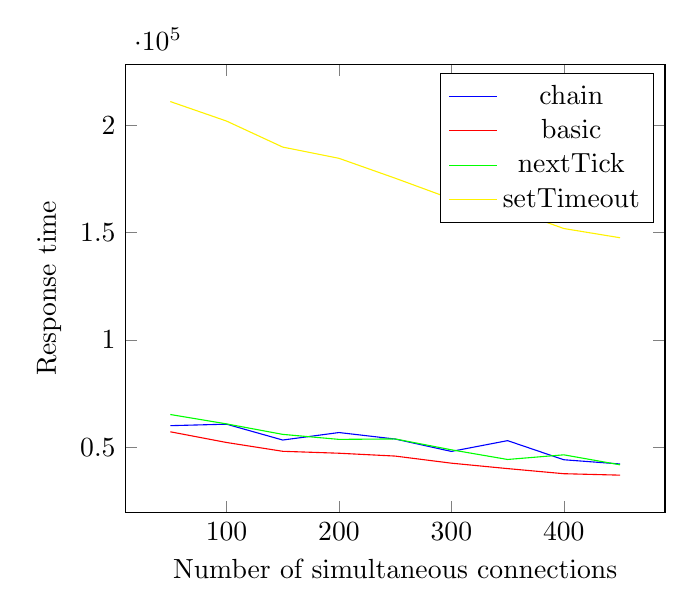
\begin{tikzpicture}
\begin{axis}[xlabel = Number of simultaneous connections, ylabel = Response time]
\addplot[color = blue] coordinates {(50, 60119.273172413814) (100, 60810.6431071428) (150, 53432.76434567901) (200, 56922.77901923074) (250, 53898.58569600001) (300, 48131.27358333333) (350, 53153.92239751554) (400, 44256.35740909089) (450, 42290.9475238095)};
\addplot[color = red] coordinates {(50, 57270.243655172475) (100, 52291.44685714285) (150, 48190.33730864198) (200, 47292.73021153844) (250, 45965.969983999996) (300, 42662.42051388889) (350, 40133.31911801241) (400, 37762.005920454554) (450, 37086.170052910056)};
\addplot[color = green] coordinates {(50, 65311.8316551724) (100, 60949.65357142856) (150, 56064.83629629629) (200, 53735.50407692306) (250, 53947.37227200004) (300, 48887.480125000024) (350, 44383.88242236024) (400, 46548.60027272731) (450, 41911.67969312167)};
\addplot[color = yellow] coordinates {(50, 210981.88593103446) (100, 201909.09617857132) (150, 189791.9731358024) (200, 184565.7975192309) (250, 175313.35167999993) (300, 165698.69973611107) (350, 161252.9545093167) (400, 151887.81970454537) (450, 147591.37962962966)};
\legend{chain, basic, nextTick, setTimeout};
\end{axis}
\end{tikzpicture}
